\begin{figure}
  \setlength{\unitlength}{\textwidth}
  \fbox{
  \begin{picture}(1,0.9)(0,0)
    % % %90
      % % % Parkinson Data 
      \put(0.035,0.5){\includegraphics[width=0.5\unitlength]{../FnP/gnuplot/displacement_amp_re200.eps}}
      \put(0.035,0.27){\includegraphics[width=0.5\unitlength]{../FnP/gnuplot/velocity_amp_re200.eps}}
      \put(0.035,0.02){\includegraphics[width=0.5\unitlength]{../FnP/gnuplot/mean_power_re_200.eps}}
      
      \put(0.495,0.27){\includegraphics[width=0.5\unitlength]{../FnP/gnuplot/velocity_amp_collapsed_re200.eps}} 
      \put(0.495,0.02){\includegraphics[width=0.5\unitlength]{../FnP/gnuplot/mean_power_collapsed_re_200.eps}}
      \put(0.495,0.5){\includegraphics[width=0.5\unitlength]{../FnP/gnuplot/displacement_amp_collpased_re200.eps}}
      
%      \put(0.23,0.00){ $\displaystyle\frac{c}{\rho\mathcal{A}U}$}
%      \put(0.73,0.00){ $\displaystyle\frac{c}{\rho\mathcal{A}U}$}

      \put(0.28,0.00){\ustar}
      \put(0.78,0.00){\massdamp}
      
      \put(0.01,0.405){$\displaystyle\frac{V}{D}$}\
       \put(0.01,0.63){$\displaystyle\frac{A}{D}$}
      
      \put(-0.02,0.13){$\displaystyle\small\frac{P_{m}}{\rho \mathcal{A}U^3 }$}
      
      \put(0.093,0.705){\small(a)}
      \put(0.555,0.705){\small(b)}
      \put(0.093,0.475){\small(c)}
      \put(0.555,0.475){\small(d)}
      \put(0.093,0.225){\small(e)}
      \put(0.555,0.225){\small(f)}

  \end{picture}
}
  \caption{Displacement amplitude, velocity amplitude and mean power data as functions of two different independent varibles. Data presented in (a), (c) and (e) using the classical VIV parameter $\ustar$, obtained at $Re=200$ and $m^*=20$ at three different damping ratios: $\zeta=0.075$ ($\times$), $\zeta=0.1$ (\ding{117}) and $\zeta=0.15$ (+). (b) (d) and (f)  are the same data presented using the combined mass-damping parameter (\massdamp) as the independent variable.  }
  \label{fig:compare_data}
\end{figure}